\documentclass[12pt]{../../oss-apphys-exam}
\usepackage{enumitem}

\usetikzlibrary{patterns}

\tikzset{
  >=latex
}

\runningheader{
  \fontfamily{phv}\small
  \textcolor{gray}{AP PHYSICS C: MECHANICS $\blacksquare$}
  \textbf{MULTIPLE-CHOICE QUESTIONS}}{}{}


\begin{document}

\begin{center}
  {
    \fontfamily{phv}\Large
    \textbf{AP PHYSICS C: MECHANICS \\SECTION I \\TIME -- 40 MINUTES}
  }
\end{center}

\textbf{Directions:} Each of the questions or incomplete statements below is
followed by five suggested answers or completions. Select the one that is best
in each case by clicking on the corresponding box directly on the web interface
with your mouse.
%and place the letter of your choice in the corresponding box on
%the student answer sheet.

\vspace{.2in}\textbf{Note:} To simplify calculations, you may use
$g=\SI{10}{\metre\per\second\squared}$ in all problems.

\begin{questions}
  \question Which of the following graphs of position $x$ versus time $t$
  corresponds to motion of an object in a straight line with positive
  acceleration?
  
  \begin{oneparchoices}
    \choice
    \begin{tikzpicture}[scale=1.2,thick]
      \draw[->] (0,0)--(2,0) node[right]{$t$};
      \draw[->] (0,0)--(0,2) node[above]{$x$};
      \draw (0,1)--(2,1);
    \end{tikzpicture}

    \choice
    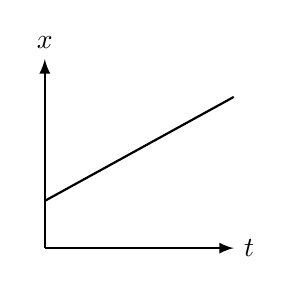
\begin{tikzpicture}[scale=1.2,thick]
      \draw[->] (0,0)--(2,0) node[right]{$t$};
      \draw[->] (0,0)--(0,2) node[above]{$x$};
      \draw (0,.5)--(2,1.6);
    \end{tikzpicture}

    \choice
    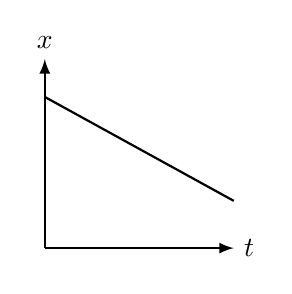
\begin{tikzpicture}[scale=1.2,thick]
      \draw[->] (0,0)--(2,0) node[right]{$t$};
      \draw[->] (0,0)--(0,2) node[above]{$x$};
      \draw (0,1.6)--(2,.5);
    \end{tikzpicture}

    \choice
    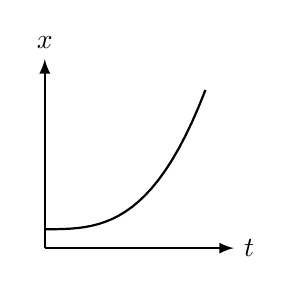
\begin{tikzpicture}[scale=1.2,thick]
      \draw[->] (0,0)--(2,0) node[right]{$t$};
      \draw[->] (0,0)--(0,2) node[above]{$x$};
      \draw[domain=0:1.7] plot(\x,{\x*\x*\x*.3+.2});
    \end{tikzpicture}

    \choice
    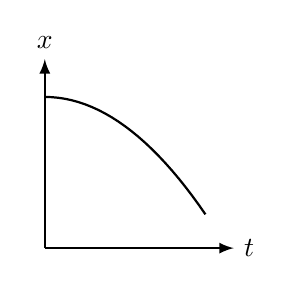
\begin{tikzpicture}[scale=1.2,thick]
      \draw[->] (0,0)--(2,0) node[right]{$t$};
      \draw[->] (0,0)--(0,2) node[above]{$x$};
      \draw[domain=0:1.7] plot(\x,{-\x*\x*.43+1.6});
    \end{tikzpicture}
  \end{oneparchoices}
  
  \question A ball is thrown straight up from a point \SI2{\metre} above the
  ground. The ball reaches a maximum height of \SI3{\metre} above its starting
  point and then falls \SI5{\metre} to the ground. When the ball strikes the
  ground, what is its displacement from its starting point?
  \begin{choices}
    \choice Zero
    \choice \SI8{\metre} below
    \choice \SI5{\metre} below
    \choice \SI2{\metre} below
    \choice \SI3{\metre} above
  \end{choices}

  % I CANNOT BELIEVE THAT THIS QUESTION MADE IT TO THE PRACTICE TEST...EVER
  %\question What do acceleration and velocity have in common?
  %\begin{choices}
  %  \choice Both are scalars.
  %  \choice Both are vectors.
  %  \choice Both are measured in units of distance divided by time.
  %  \choice Both are measured in units of distance divided by time squared.
  %  \choice They are different names for the same quantity.
  %\end{choices}


  \question A particle is moving along the $y$-axis. The particle's position as
  a function of time is given by $y=\alpha t^3-\beta t+\varphi$, where
  $\alpha=\SI1{\metre\per\second\cubed}$, $\beta=\SI4{\metre\per\second}$, and
  $\varphi=\SI3\metre$. What is the particle's acceleration at time
  $t=\SI3\second$?
  \begin{choices}
    \choice\SI{6.0}{\metre\per\second\squared}
    \choice\SI{9.0}{\metre\per\second\squared}
    \choice\SI{18}{\metre\per\second\squared}
    \choice\SI{23}{\metre\per\second\squared}
    \choice\SI{27}{\metre\per\second\squared}
  \end{choices}
  \newpage
  
  \question Two projectiles are launched with the same initial speed from the
  same location, one at a \ang{30} angle and the other at a \ang{60} angle with
  the horizontal. They land at the same height at which they were launched. If
  air resistance is negligible, how do the projectiles' respective maximum
  heights, $H_{30}$ and $H_{60}$ , and times in the air, $T_{30}$ and $T_{60}$,
  compare with each other?

  \begin{tabular}{ccc}
    & Maximum Height & Time in Air \\ \hline
    (A) & $H_{30} > H_{60}$ & $T_{30} > T_{60}$ \\
    (B) & $H_{30} > H_{60}$ & $T_{30} < T_{60}$ \\
    (C) & $H_{30} = H_{60}$ & $T_{30} = T_{60}$ \\
    (D) & $H_{30} < H_{60}$ & $T_{30} > T_{60}$ \\
    (E) & $H_{30} < H_{60}$ & $T_{30} < T_{60}$
  \end{tabular}

  \uplevel{
    \textbf{Questions \ref{proj1}--\ref{proj2}}
    \cpic{.35}{projectile1}
    A rock is thrown from the edge of a cliff with an initial velocity $v_0$ at
    an angle $\theta$ with the horizontal as shown above. Point $P$ is the
    highest point in the rock's trajectory and point $Q$ is level with the
    starting point. Assume air resistance is negligible.
  }

  \question Which of the following correctly describes the horizontal and
  vertical speeds and the acceleration of the rock at $P$?
  \label{proj1}

  \begin{tabular}{cccc}
    & Horizontal Speed & Vertical Speed & Acceleration \\ \hline
    (A)  & $v_0\cos\theta$ & 0 & $g$ \\
    (B)  & 0               & 0 & $g$ \\
    (C)  & $v_0\cos\theta$ & 0 & 0   \\
    (D)  & $v_0\cos\theta$ & $v_0\sin\theta$ & 0   \\
    (E)  & 0 & $v_0\cos\theta$ & 0
  \end{tabular}

  \question Which of the following correctly describes the horizontal and
  vertical speeds and the acceleration of the rock at $Q$?
  \label{proj2}

  \begin{tabular}{cccc}
    & Horizontal Speed & Vertical Speed & Acceleration \\ \hline
    (A)  & $v_0\cos\theta$ & 0 & $g$ \\
    (B)  & 0               & 0 & $g$ \\
    (C)  & $v_0\cos\theta$ & 0 & 0   \\
    (D)  & $v_0\cos\theta$ & $v_0\sin\theta$ & 0   \\
    (E)  & 0 & $v_0\cos\theta$ & 0
  \end{tabular}
  \newpage
  
  \question An object of mass \SI{100}{\kilo\gram} is initially at rest on a
  horizontal frictionless surface. At time $t=0$, a horizontal force of
  \SI{10}{\newton} is applied to the object for \SI1{\second} and then
  removed. Which of the following is true of the object at time
  $t=\SI2\second$ if it is still on the surface?
  \begin{choices}
    \choice It is at the same position it had at $t=0$, since a force of
    \SI{10}{\newton} is not large enough to move such a massive object.
    \choice It is moving with constant nonzero acceleration.
    \choice It is moving with decreasing acceleration.
    \choice It is moving at a constant velocity.
    \choice It has come to rest some distance away from the position it had at
    $t=0$.
  \end{choices}
  
  \question Several forces act on an object, but the object is in equilibrium.
  Which of the following statements about the object \emph{must} be true?
  \begin{enumerate}[nosep]
  \item[I.] It has zero acceleration.
  \item[II.] The net force acting on it is zero.
  \item[III.] It is at rest.
  \item[IV.] It is moving with constant velocity.
  \end{enumerate}
  \begin{choices}
    \choice I and II
    \choice I and III
    \choice I and IV
    \choice II and III
    \choice II and IV
  \end{choices}
 
  \uplevel{
    \textbf{Questions \ref{toycar1}--\ref{toycar2}}
    
    A toy car of mass 6 kg, moving in a straight path, experiences a net force
    given by the function $F=-3t$. At time $t=0$, the car has a velocity of
    \SI{4}{\metre\per\second} in the positive direction and is located
    $+8$ \si{\metre} from the origin.
  }
  
  \question The car will come instantaneously to rest at time $t$ equal to
  \label{toycar1}  
  \begin{choices}
    \choice$\dfrac23$ \si\second
    \choice$\sqrt{\dfrac43}$ \si\second
    \choice$\sqrt{\dfrac83}$ \si\second
    \choice$\sqrt8$ \si\second
    \choice\SI{4}{\second}
  \end{choices}

  \question Which of the following best shows a graph of position $d$ versus
  time $t$ for the car?
  
  \begin{oneparchoices}
    \choice
    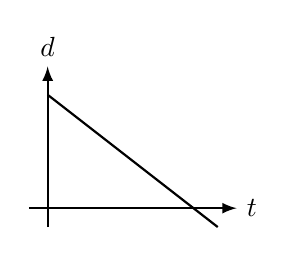
\begin{tikzpicture}[scale=1.2,thick]
      \draw[->] (-.2,0)--(2,0) node[right]{$t$};
      \draw[->] (0,-.2)--(0,1.5) node[above]{$d$};
      \draw (0,1.2)--(1.8,-.2);
    \end{tikzpicture}

    \choice
    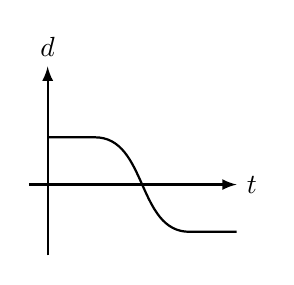
\begin{tikzpicture}[scale=1.2,thick]
      \draw[->] (-.2,0)--(2,0) node[right]{$t$};
      \draw[->] (0,-.75)--(0,1.25) node[above]{$d$};
      \draw (0,.5)--(.5,.5) to[out=0,in=180] (1.5,-.5)--(2,-.5);
    \end{tikzpicture}

    \choice
    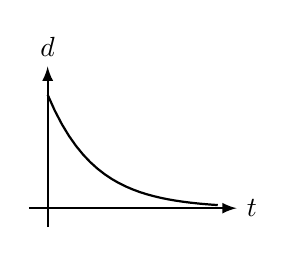
\begin{tikzpicture}[scale=1.2,thick]
      \draw[->] (-.2,0)--(2,0) node[right]{$t$};
      \draw[->] (0,-.2)--(0,1.5) node[above]{$d$};
      \draw[domain=0:1.8] plot(\x,{1.2*exp(-2*\x)});
    \end{tikzpicture}
    
    \choice
    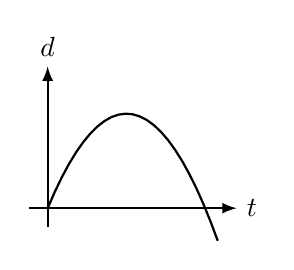
\begin{tikzpicture}[scale=1.2,thick]
      \draw[->] (-.2,0)--(2,0) node[right]{$t$};
      \draw[->] (0,-.2)--(0,1.5) node[above]{$d$};
      \draw[domain=0:1.8] plot(\x,{-4*(.6*\x-.5)*(.6*\x-.5)+1});
    \end{tikzpicture}

    \choice
    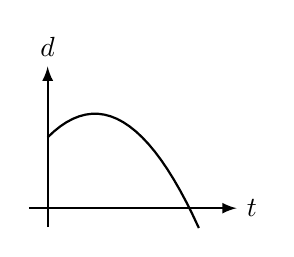
\begin{tikzpicture}[scale=1.2,thick]
      \draw[->] (-.2,0)--(2,0) node[right]{$t$};
      \draw[->] (0,-.2)--(0,1.5) node[above]{$d$};
      \draw[domain=0:1.6] plot(\x,{-(\x-.5)*(\x-.5)+1});
    \end{tikzpicture}
  \end{oneparchoices}
  \label{toycar2}


  \uplevel{
    \textbf{Questions \ref{slowdown1}--\ref{slowdown2}}
      
    An object of mass 0.5 kg is given an initial velocity and then slides
    across a horizontal surface. The object experiences a resistive force that
    is a function of  velocity. The velocity v of the object as a function
    of time $t$ is given by $v(t)=\alpha e^{-\beta t}$ , where
    $\alpha=\SI2{\metre\per\second}$ and $\beta=\SI3{\per\second}$.
  }
  \question Which of the following is a correct expression for the net force,
  in newtons, exerted on the object as a function of time?
  \label{slowdown1}
  \begin{choices}
    \choice $-6e^{-3t}$
    \choice $-3e^{-3t}$
    \choice $e^{-3t}$
    \choice $2e^{-3t}$
    \choice $\dfrac2{3\left(1-e^{-3t}\right)}$
  \end{choices}

  \question The energy dissipated due to the resistive force after a very long
  time is most nearly
  \label{slowdown2}
  \begin{choices}
    \choice 0.5 J
    \choice 1 J
    \choice 2 J
    \choice 4 J
    \choice infinity
  \end{choices}

  \uplevel{
    \centering
    \begin{tikzpicture}
      \fill[lightgray] rectangle (5.5,-.3);
      \draw[very thick] (0,0)--(5.5,0);
      \draw[thick] (.5,0) rectangle +(3,.7);
      \draw[thick] (1.2,.7) rectangle +(1.5,.7);
      \draw[vectors] (3.5,.35)--+(1.5,0) node[right]{$\vec F$};
    \end{tikzpicture}
  }
  \question Two blocks rest on a table, as shown above. The bottom block is
  pulled to the right by an applied force $\vec F$ that is strong enough so
  that the two blocks \underline{do not move together} (i.e.\ they do not have
  the same acceleration or velocity). There is friction between the blocks, but
  the tabletop is frictionless. When the top block leaves the bottom block,
  where does it land and why?
  \begin{choices}
    \choice The top block will land directly below where it starts because
    objects at rest tend to stay at rest.

    \choice The top block will land to the left of where it starts because of
    the static friction between the blocks.
    
    \choice The top block will land to the left of where it starts because of
    the kinetic friction between the blocks.
    
    \choice The top block will land to the right of where it starts because of
    the static friction between the blocks.
    
    \choice The top block will land to the right of where it starts because of
    the kinetic friction between the blocks.
  \end{choices}
  \newpage
  
  \uplevel{
    \textbf{Questions \ref{connect1}--\ref{connect2}}
    \cpic{.28}{connected-mass}
    A block of mass $M_1$ on a horizontal table is connected to a hanging block
    of mass $M_2$ by a string that passes over a pulley, as shown above. The
    acceleration of the blocks is $0.6g$. Assume that friction and the mass of
    the string are negligible.
  }

  \question The tension $T$ in the string is \label{connect1}
  \begin{choices}
    \choice zero
    \choice $0.4M_2g$
    \choice $0.6M_2g$
    \choice $1.0M_2g$
    \choice $1.6M_2g$
  \end{choices}
  
  \question The ratio of masses $M_2/M_1$ is  \label{connect2}
  \begin{choices}
    \choice 0.67
    \choice 1.0
    \choice 1.4
    \choice 1.5
    \choice 1.6
  \end{choices}

  \uplevel{
    \textbf{Questions \ref{spring1}--\ref{spring2}}
    \cpic{.28}{spring-mass}
    \vspace{-.1in}In the system of two blocks and a spring shown above, blocks
    1 and 2 are
    connected by a string that passes over a pulley. The initially unstretched
    spring connects block 1 to a rigid wall. Block 1 is released from rest,
    initially slides to the right, and is eventually brought to rest by the
    spring and by friction on the horizontal surface.
  }

  \question Which of the following is true of the energy of the system during
  this process?
  \begin{choices}
    \choice The total mechanical energy of the system is conserved.
    \choice The total mechanical energy of the system increases.
    \choice The energy lost to friction is equal to the gain in the potential
    energy of the spring.
    \choice  The potential energy lost by block 2 is less in magnitude than the
    potential energy gained by the spring.
    \choice The potential energy lost by block 2 is greater in magnitude than
    the potential energy gained by the spring.
  \end{choices}
  \label{spring1}

  \question After block 1 comes to rest, the force exerted on it by the spring
  must be equal in magnitude to
  \begin{choices}
    \choice zero
    \choice the frictional force on block 1
    \choice the vector sum of the forces on block 1 due to friction and tension
    in the string
    \choice the sum of the weights of the two blocks
    \choice the difference in the weights of the two blocks
  \end{choices}
  \label{spring2}
  
  \uplevel{
    \centering
    \begin{tabular}{|c|c|}
      \hline
      $x$ (m) & $F$ (N) \\ \hline
      0 & 0  \\ \hline
      1 & 1  \\ \hline
      2 & 8  \\ \hline
      3 & 27 \\ \hline
      4 & 64 \\ \hline
    \end{tabular}
  }
  \question A specially designed spring is stretched from equilibrium to the
  distances $x$ given in the table above, and the restoring force $F$ is
  measured and recorded in each case. What is the potential energy of the
  spring when it is stretched \SI3{\metre} from equilibrium?
  \begin{choices}
    \choice $\dfrac92$ \si\joule
    \choice \SI9\joule
    \choice $\dfrac{81}4$ \si\joule
    \choice \SI{27}{\joule}
    \choice $\dfrac{81}2$ \si\joule
  \end{choices}
  
  \question When a certain spring is stretched by an amount $x$, it produces a
  restoring force of $F(x)=-ax+bx^2$, where $a$ and $b$ are constants. How much
  work is done by an external force in stretching the spring by an amount $D$
  from its equilibrium length?
  \begin{choices}
    \choice $-aD + bD^2$
    \choice $a - 2bD$
    \choice $\dfrac12aD^2-\dfrac13 bD^3$
    \choice $-aD^2 + bD^3$
    \choice $-2aD^2 + 3bD^3$
  \end{choices}

 \uplevel{
    \begin{center}
      \begin{tikzpicture}[scale=1.3]
        \draw[axes] (0,0)--(4.5,0) node[right]{$x$ [m]};
        \draw[axes] (0,-1.5)--(0,2.3) node[above]{$U(x)$ [J]};
        \foreach \x in {.5,1,...,4} \draw (\x,.05)--+(0,-.1);
        \foreach \x in {1,...,4} \node[below] at (\x,-.05) {$\x$};
        \foreach \y in {-1,...,2} \draw (.05,\y)--+(-.1,0) node[left]{$\y$};
        \fill (0,2) circle (.05) node[right]{$P$};
        \fill (.5,1) circle (.05);
        \fill (2,-1) circle (.05);
        \fill (4,0) circle (.05);
        \draw[very thick] (0,2)--(1,0) to[out=-atan(2),in=180] (2,-1)
        to[out=0,in=220] (4,0);
      \end{tikzpicture}
    \end{center}
    \textbf{Questions \ref{conserve1}--\ref{conserve2}} refer to the potential
    energy $U$ vs.\ position $x$ graph shown above for a particle moving in one
    dimension. All forces acting on the particle is conservative. The graph
    begins at point $P$. The kinetic energy of the particle at position $x=2$
    is \SI{3.0}\joule.
    %The graph is represented by a straight, diagonal line
    %between $x=3$ and $x=4$.
  }

  \question The magnitude of the force acting on the particle between $x=3$ and
  $x=4$ is
  \label{conserve1}
  \begin{choices}
    \choice zero
    \choice constant
    \choice increasing
    \choice decreasing
    \choice equal to the weight of the particle
  \end{choices}

  \question Which of the following statements is true of the particle?
  \label{conserve2}
  \begin{choices}
    \choice The particle is at rest at $x=2$.
    \choice The total energy of the particle at $x=2$ is \SI{+2}\joule.
    \choice The particle has enough energy to reach $x=1$.
    \choice The particle does not have enough energy to reach $x=3$.
    \choice The particle does not have enough energy to reach point $P$.
  \end{choices}
  
  \question An electron travels in a circle around a hydrogen nucleus at a very
  high  speed. The work done by the electrostatic force acting on the electron
  after one complete revolution is
  \begin{choices}
    \choice zero
    \choice positive
    \choice negative
    \choice equal to the kinetic energy of the electron
    \choice equal to the potential energy of the electron
  \end{choices}

  \uplevel{
    \centering
    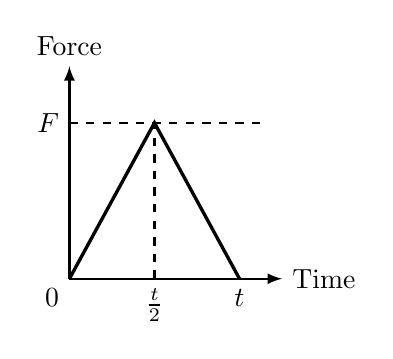
\begin{tikzpicture}[scale=.9,thick]
      \draw[->] (0,0)--(3,0) node[right]{Time};
      \draw[->] (0,0)--(0,3) node[pos=0,below left]{0} node[above]{Force};
      \draw[dashed] (0,2.2)--(2.8,2.2) node[pos=0,left]{$F$};
      \draw[dashed] (1.2,0)--(1.2,2.2) node[pos=0,below]{$\frac t2$};
      \draw[very thick] (0,0)--(1.2,2.2)--(2.4,0) node[below]{$t$};
    \end{tikzpicture}
  }
  \question\vspace{-.1in}The graph above shows the force acting on an object as
  a function of time. The change in momentum of the object from time 0 to $t$ is
  \begin{choices}
    \choice $2Ft$
    \choice $Ft$
    \choice $\dfrac12Ft$
    \choice $\dfrac14Ft$
    \choice zero
  \end{choices}
  
  \question A toy spacecraft is launched directly upward. When the toy reaches
  its highest point, a spring is released and the toy splits into two parts
  with masses of \SI{.02}{\kilo\gram} and \SI{.08}{\kilo\gram}, respectively.
  Immediately after the separation, the \SI{.02}{\kilo\gram} part moves
  horizontally due east. Air resistance is negligible. True statements about
  the \SI{.08}{\kilo\gram} part include which of the following?
  \begin{enumerate}[nosep]
  \item[I.] It could move north immediately after the spring is released.
  \item[II.] It takes longer to reach the ground than does the
    \SI{.02}{\kilo\gram} part.
  \item[III.] It strikes the ground farther from the launch point than does the
    \SI{.02}{\kilo\gram} part.
  \end{enumerate}
  \begin{choices}
    \choice None
    \choice I only
    \choice III only
    \choice I and II only
    \choice II and III only
  \end{choices}

  \uplevel{
    \cpic{.45}{child}
  }
  
  \question As shown in the figure above, a child of mass \SI{20}{\kilo\gram}
  who is running at a speed of \SI{4.0}{\metre\per\second} jumps onto a
  stationary sled of mass \SI{5.0}{\kilo\gram} on a frozen lake. The speed at
  which the child and sled begin to slide across the ice is most nearly
  \begin{choices}
    \choice \SI{.20}{\metre\per\second}
    \choice \SI{.80}{\metre\per\second}
    \choice \SI{1.2}{\metre\per\second}
    \choice \SI{3.2}{\metre\per\second}
    \choice \SI{16}{\metre\per\second}
  \end{choices}
\end{questions}
\end{document}
